% general format definition
\documentclass[a4paper, 11pt]{article}
\usepackage[margin=.9in]{geometry}
\usepackage[utf8]{inputenc}
\usepackage[T1]{fontenc}
\usepackage[english]{babel}

% extra packages
\usepackage{hyperref}
\usepackage{listings}
\usepackage{color}
\usepackage{amssymb}
\usepackage{amsmath}
\usepackage{mathtools}
\usepackage{microtype}
\usepackage{stmaryrd}
\usepackage{tikz}
\usepackage{booktabs}
\usepackage{stmaryrd}

% special math symbols
\newcommand{\R}{\ensuremath{\mathbb{R}}}
\newcommand{\N}{\ensuremath{\mathbb{N}}}
\newcommand{\Z}{\ensuremath{\mathbb{Z}}}
\newcommand{\Q}{\ensuremath{\mathbb{Q}}}

% Fraktur für Strukturen
\newcommand{\A}{\ensuremath{\mathfrak A}}
\newcommand{\B}{\ensuremath{\mathfrak B}}
\newcommand{\C}{\ensuremath{\mathfrak C}}
\newcommand{\I}{\ensuremath{\mathfrak I}}

% logical operators
\newcommand{\xor}{\ensuremath{\oplus}} %exklusives oder
\newcommand{\impl}{\ensuremath{\rightarrow}} %logische Implikation

% nicer symbols
\renewcommand{\phi}{\varphi}
\renewcommand{\theta}{\vartheta}
\renewcommand{\epsilon}{\varepsilon}

% Syntax highlighting
\definecolor{commentsColor}{rgb}{0.497495, 0.497587, 0.497464}
\definecolor{keywordsColor}{rgb}{0.000000, 0.000000, 0.635294}
\definecolor{stringColor}{rgb}{0.558215, 0.000000, 0.135316}
\lstset{
  backgroundcolor=\color{white},                        % choose the background color; you must add \usepackage{color} or \usepackage{xcolor}
  basicstyle=\footnotesize,                             % the size of the fonts that are used for the code
  breakatwhitespace=false,                              % sets if automatic breaks should only happen at whitespace
  breaklines=true,                                      % sets automatic line breaking
  captionpos=b,                                         % sets the caption-position to bottom
  commentstyle=\color{commentsColor}\textit,            % comment style
  deletekeywords={},                                    % if you want to delete keywords from the given language
  escapeinside={\%*}{*)},                               % if you want to add LaTeX within your code
  extendedchars=true,                                   % lets you use non-ASCII characters; for 8-bits encodings only, does not work with UTF-8
  frame=tb,	                   	                    % adds a frame around the code
  keepspaces=true,                                      % keeps spaces in text, useful for keeping indentation of code (possibly needs columns=flexible)
  keywordstyle=\color{keywordsColor}\bfseries,          % keyword style
  otherkeywords={True,False,true,false,null,None,NULL,exit,wait,fork,*,&}, % if you want to add more keywords to the set
  numbers=left,                                         % where to put the line-numbers; possible values are (none, left, right)
  numbersep=5pt,                                        % how far the line-numbers are from the code
  numberstyle=\tiny\color{commentsColor},               % the style that is used for the line-numbers
  rulecolor=\color{black},                              % if not set, the frame-color may be changed on line-breaks within not-black text (e.g. comments (green here))
  showspaces=false,                                     % show spaces everywhere adding particular underscores; it overrides 'showstringspaces'
  showstringspaces=false,                               % underline spaces within strings only
  showtabs=false,                                       % show tabs within strings adding particular underscores
  stepnumber=1,                                         % the step between two line-numbers. If it's 1, each line will be numbered
  stringstyle=\color{stringColor},                      % string literal style
  tabsize=2,	                                      % sets default tabsize to 2 spaces
  title=\lstname,                                       % show the filename of files included with \lstinputlisting; also try caption instead of title
  columns=fixed,                                        % Using fixed column width (for e.g. nice alignment)
  language=c
}

\author{Thilo Metzlaff\\406247 \and Mats Frenk\\393702\and René van Emelen\\406008}
\title{BUS Exercise 3 \\ Group 23}
\begin{document}
    % titlepage
    \maketitle
    \newpage

    % contents
    \tableofcontents
    \newpage

    % section 0
    \section*{Introduction}
    Welcome back to this special endeavour, where i write every single thing in \LaTeX{}; Please be patient, while we look for the missing full-stop and enjoy a semicolon instead.\\
    Now... How was it that i defined all this again? Lemme look for the definition real quick\dots\\
    Ah yes, there it is:

    \subsection*{THE FORMAT}
    \begin{itemize}
        \item Every file will be named similar to the sections in here, so\\
              \texttt{2.1-stack\_exercise.c} is Exercise 2, section 1.
        \item Every Solution \textbf{WILL} be in this pdf, but not necessarily 
              anything predefined by the exercise.
        \item Any explanation will be both in this PDF as well as in each file.
        \item This explanation will be in each PDF, in case someone who doesn't
              know the format tries to correct the exercises
        \item \textbf{WARNING:} Humor may or may not be used. If you are allergic
              to humor, that sounds like a personal problem.
    \end{itemize}
    \newpage

    % Section 1
    \section{Linux Processes and Child creation}
    
    \subsection{Controlled Forking}
    To control the output of parent and child, we need another \texttt{if-else} construct, testing the return value of 
    \texttt{fork()}. If said value is 0, we are in the child and we can execute \texttt{child\_B\_proc()}, otherwise we 
    execute \texttt{child\_A\_proc()}. The final code looks like this:
    \lstinputlisting{3.1_prozesse.c}
    \newpage
    
    \subsection{Streams}
    \texttt{stdin} and \texttt{stdout} are so-called "streams". A stream is a  temporary memory space that we can
    use to write to and communicate. This ensures that we only write to a specific location and only when data is complete. \texttt{stdin} and \texttt{stdout}
    are the program's IO streams. Reading from \texttt{stdin} will read any input that has been given to a program
    and reading \texttt{stdout} wil give its output. That is how the linux terminal reads the program's output as well.\\
    The problem in a stream is the fact that they persist, unless we manually flush them.
    So writing "\texttt{aaaaaaaaa}" into \texttt{stdout} and then writing "\texttt{test}" to it,
    will result in the outputs "\texttt{aaaaaaaaa}" and "\texttt{testaaaaa}", because we overwrite the stream without flushing it.
    That's why you should firs to flush any stream before writing to it.\\
    \lstinline{printf(char*, \dots)} and \lstinline{fprintf(char* buf, char*,...)} don't flush, but rather they pad the output to the next 
    byte and add a \lstinline{NULL} terminator instead. To prevent this, we can use \lstinline{fflush(buf)} and completely flush the stream.
    Both functions also parse the string to look for formatting and where to insert variables, before using \lstinline{write(int fd, char* buf, int blen);} 
    In this case, \texttt{write()} is more efficient, because \texttt{write()} doesn't check the string. It writes it to stdout.
    
    \subsection{Undead Processes}
    A Zombie process is simply said: a process with daddy issues.\\
    Zombie processes are created, when the child's Process Descriptor isn't updated in the parent process and the child terminates unexpectedly.
    In this case, the prozess is dead, but its descriptor still exists, so the parent thinks the process is still running and leaves it registered.
    To prevent this, one can simply use the \texttt{wait()} and \texttt{exit()} syscalls, this makes the parent wait and update the Status of the child
    as soon as it commits suicide (terminates) with \texttt{exit()};

    \subsection{Linking Children}
    A child process always has its parent's PID linked, so it can be identified by the system and organized appropriately. 
    If this wasn't the case, the system couldn't create a proper process tree structure and would fail to execute a program. 

    \subsection{Parent/Child execution priority}
    Using the program \texttt{charcount.c}, one can pipe \texttt{prozesse.c} into it and observe, that the percentage frequency is approximately $30\%$.
    This percentage drifts around, due to the random execution order. In long term observation, one can see that the frequency will drift further, suddenly prioritizing
    a single process A LOT stronger, but then changing between them. The conclusion would be, that, on average, all processes have the same priority and frequency.
    \newpage
    \lstinputlisting{3.1_charcounter.c}
    \newpage

    \section{Tree Hugging}
    
    \subsection{The Family Tree}
    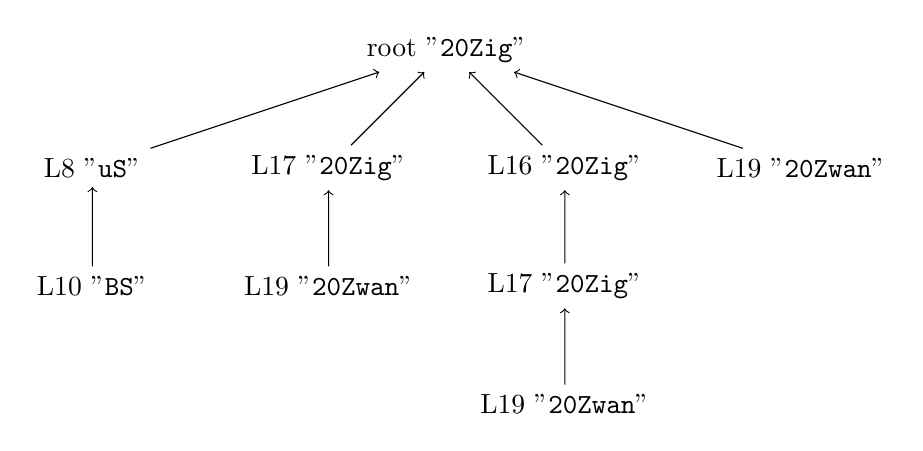
\begin{tikzpicture}[<-, level distance=1.5cm,
    level 1/.style={sibling distance=3cm},
    level 2/.style={sibling distance=2.5cm}]
          \node {root "\texttt{20Zig}"}
                child { node {L8 "\texttt{uS}"}
                      child{ node {L10 "\texttt{BS}"}}
                }
                child { node { L17 "\texttt{20Zig}"}
                      child{ node {L19 "\texttt{20Zwan}"}}
                }
                child { node {L16 "\texttt{20Zig}"}
                      child { node { L17 "\texttt{20Zig}"}
                            child{ node {L19 "\texttt{20Zwan}"}}
                      }
                }
                child{ node {L19 "\texttt{20Zwan}"}}
                ;
    \end{tikzpicture}

    \subsection{Parent-Child execution order}
    The child process and the parent process have the same priority. Therefore the OS has to decide which process to execute first, by randomly chosing.
    This makes the order of execution random, unless the parent awaits the child process's execution. 

    \subsection{Wait for Order 66}
    Since we want a deterministic program output, namely "\texttt{BuS 20ZwanZig}", we have to wait for each child to do its thing.
    How does one wait for a child to terminate itself, you might ask? Simply by using \lstinline{exit(0);} in the child process. 
    To use wait and exit, we have to do \lstinline{#include <stdlib.h>} and \lstinline{#include <sys/wait.h>}.
    Now we are able to use \lstinline{wait} and \lstinline{exit}.\\
    Since we can just use \lstinline{wait(NULL);} to block a parent until all children are done, we just use that a bunch of times.
    Before we can get a fully deterministic output, we have to end some processes early, to only get the unique output. we can do 
    this by checking if \lstinline{fork();} returned 0, meaning we are in a child, and then terminating early. I terminated all child
    processes before the 20, they are useless here, because they give duplicate output.  
    \newpage
    \lstinputlisting{3.2_fork.c}
    \newpage

    \section{Process data communism}
      Due to personal time management issues, i admit that i copied this exercise from a friend, after we agreed that the solution is likely correct.
      This was solved in collaboration, i just didn't have the time to reformulate it in my own words.
      \subsection{Stuffing things in Pipes or cooperative memory use?}
      \begin{table}[h]
            \begin{tabular}{@{}llll@{}}
                  \multicolumn{4}{c}{Pipes}                                                                                      \\
                  \multicolumn{2}{c}{+}                         & \multicolumn{2}{c}{-}                                          \\ \midrule
                  \multicolumn{2}{l|}{- simple synchronisation} & \multicolumn{2}{l}{- one-to-one communication only}            \\
                  \multicolumn{2}{l|}{- easy debugging}         & \multicolumn{2}{l}{- OS driven and therefore not customizable} \\
                  \multicolumn{2}{l|}{- easy to implement}      & \multicolumn{2}{l}{}                                          
            \end{tabular}
      \end{table}

      \begin{table}[h]
            \begin{tabular}{@{}llll@{}}
                  \multicolumn{4}{c}{Shared Memory}                                                                                      \\
                  \multicolumn{2}{c}{+}                         & \multicolumn{2}{c}{-}                                          \\ \midrule
                  \multicolumn{2}{l|}{- asynchronous} & \multicolumn{2}{l}{- code can be pretty complex}            \\
                  \multicolumn{2}{l|}{- more than two connections possible} & \multicolumn{2}{l}{- hard to debug} \\
                  \multicolumn{2}{l|}{- fast}      & \multicolumn{2}{l}{}                                          
            \end{tabular}
      \end{table}
      \subsection{}
      Shared Memory: \\
      Hier müsste man ein Segment im Speicher einrichten, welches die Daten aus dem Firefoxfenster nimmt und diese von der Konsole über dieses Segment im Speicher gelesen werden.
      Dies beinhaltet einen großen Programmieraufwand, da die Kommunikation asynchron abläuft.\\
      Message Passing:\\
      Hier wird eine linked List im Kernel gespeichert, welche die Informationen des Firefox Fensters aufnimmt und dann abspeichert. Diese können von der Konsole ausgelesen werden.
      Auch diese Kommunikationsform wäre asynchron, aber dafür im System vordefiniert. Außerdem ist diese Kommunikationform Bidirektional, was hier jedoch nicht verwendet wird.
      \\
      Pipes:\\
      Hier ergeben Pipes am meisten Sinn, da diese synchron arbeiten, keinen Programmieraufwand benötigen, da es in allen Systemen standardisiert ist, und
      auch unidirektional benötigt werden können. Dies ist praktisch, weil man vom Konsolenfenster keine Daten lesen muss und entsprechend auch keinen Aufwand betreiben muss, diese Datenverbindungen zu timen.
      \newpage
      \subsection{}
      Ein Thread ist ein Subset eines Prozesses. Dabei kann jeder Prozess einen oder mehrere Threads haben. Dies bezeichnet einfach nur, dass ein Codesegment auf mehreren Threads laufen kann und damit die Execution-Time verringert wird.
      Da Threads shared Memory besitzen, ist der Austausch zwischen Threads leichter als zwischen isolierten Prozessen.
      \subsection*{}
      Erhält ein Prozess mehr Softwarethreads als der Computer Hardwarethreads besitzt, so findet $time \mbox{ } slicing$ statt. $time \mbox{ } slicing$ bewirkt, dass jeder Thread einen spezifischen time frame erhält, in welchem er das entsprechende Code-Segment ausführen kann. Dies führt aber zu einem Delay in der Gesamtzeit, weil dann zwischen Threads abgewechselt werden muss, statt sie parallel laufen zu lassen.

\end{document}